\chapter{Análise de requisitos}

A análise dos requisitos dun produto software é unha parte fundamental do proceso de desenvolvemento, pois consiste definir de forma detallada o que debe facer o produto para satisfacer as necesidades e cumprir as expectativas do cliente.

O proceso de xestión de requisitos\cite{GPGR} consistirá en definir conxuntamente co cliente os distintos casos de uso do software. A partir dos casos de uso identificados extráense e documéntanse os requisitos, que se usarán como referencia para o desenvolvemento do sistema.

\section{Casos de uso}

Os casos de uso\cite{UseCase} describen as interaccións entre os actores é o sistema nunha linguaxe non técnica, centrándose en que fai sistema para o actor, entendendo por actor calquera entidade externa o sistema que lle demanda algunha funcionalidade.

Neste proxecto identifícase un único actor, que é o usuario xenérico da aplicación, pois nin existen distintos roles de usuarios nin outras entidades externas.

A continuación descríbense os casos de uso identificados en colaboración co cliente, e que se resumen graficamente na figura \ref{fig:uc}.

\uctable 	{CU.01}{Consultar as capacidades dun servidor SOS}
			{Consultar as capacidades dun servidor SOS para ver as ofertas que realiza e as propiedades dispoñibles nelas, e demais información do servizo.} %Propósito
			{É estendido polo \ref{uc:CU.02}} %Relacións
			{-} %Precondicións 
			{Visualízanse as capacidades do SOS nun formato amigable para o usuario.} %Postcondicións
			{O usuario introduce o enderezo do servidor SOS, ou selecciónao de entre os gardados. A aplicación descarga as capacidades do mesmo para amosalas en pantalla. 
			} %Escenario
			
\uctable 	{CU.02}{Obter observacións do servidor SOS}
			{Xerar unha capa vectorial cos datos das observacións rexistradas no SOS.} %Propósito
			{Estende o \ref{uc:CU.01}} %Relacións
			{Ter consultado as capacidades do servizo.} %Precondicións 
			{Capa vectorial coas observacións obtidas.} %Postcondicións
			{O usuario crea selecciona a través da interface gráfica a oferta e propiedades a consultar, así como outros filtros máis avanzados, por entidade de interese, sensor, período de tempo, filtros espaciais, etc. A aplicación descarga as observacións e xera unha capa vectorial en QGIS coa información procesada.
			} %Escenario

\uctable 	{CU.03}{Visualizar gráficas en dúas dimensións}
			{Visualizar nunha gráfica en dúas dimensións a información das observacións a partir da capa xerada. Débese poder visualizar a evolución de unha propiedade o con respecto ó tempo, e tamén sería de utilidade en algúns caso poder enfrontar unha propiedade contra outra. } %Propósito
			{-} %Relacións
			{Ter xerada unha capa con datos de observacións.} %Precondicións 
			{Gráfico en dúas dimensións dos datos seleccionados.} %Postcondicións
			{Sobre a capa xerada o usuario seleccionará entidades de interese para poder visualizar nunha nova ventá un gráfico que represente o tempo no eixo X e a propiedade indicada no eixo Y. O usuario pode seleccionar outra propiedade para representar en cada un dos eixos.
			} %Escenario
			
\uctable 	{CU.04}{Visualizar mapas animados}
			{Facer visualizacións animadas dos datos da capa sobre o propio visor de mapas de QGIS.} %Propósito
			{-} %Relacións
			{Ter xerada unha capa con datos de observacións.} %Precondicións 
			{Visualización animada das observacións.} %Postcondicións
			{O usuario disporá duns controis de reprodución para as capas con datos de observacións de xeito que poda reproducir a evolución cronolóxica das observacións sobre o propio visor de mapas de QGIS. 
			} %Escenario

\begin{figure}[hbtp]
\centering
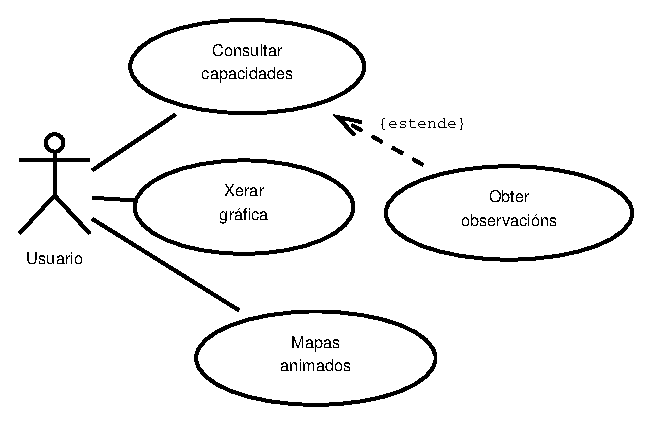
\includegraphics[scale=1]{images/uc.eps}
\caption{Diagrama de casos de uso}
\label{fig:uc} 
\end{figure}

\section{Catálogo de requisitos}
A partir dos casos de uso documentados realizase a extracción dos requisitos da aplicación. Estes requisitos son as características que debe presentar a aplicación, e definen o software desde o punto de vista do cliente. Dividimos os catálogo de requisitos en dúas partes, segundo a natureza dos mesmos:
\begin{description}
\item[Funcionais:] Son as características da aplicación para proporcionar a funcionalidade requirida.
\item[Non funcionais:] Non describen funcionalidades, se non que representan outras necesidades como seguridade, rendemento, usabilidade, ou restricións de plataforma, tecnolóxicas, e similares.
\end{description}

Clasificaremos os requisitos pola súa relevancia segundo o cadro \ref{tab:relevanciaReq}, que se terá en conta na planificación dos sprints.
\begin{table}
\begin{tabularx}{\textwidth}{lX} \toprule
	Relevancia & Descrición \\
	\midrule
	Esixido & Requisito que está directamente relacionado co cumprimento dos obxectivos do proxecto.\\
	Desexado & Requisito que mellora a calidade do proxecto, pero non está relacionado directamente cos obxectivos do mesmo.\\
	Opcional &  Requisito que non supón unha mellora substancial na calidade do proxecto, aínda que si resulta de utilidade.\\
	\bottomrule
\end{tabularx}
\caption{Niveis de relevancia dun requisito}
\label{tab:relevanciaReq}
\end{table}

\subsection{Requisitos funcionais}
Os requisitos funcionais definidos, verificados e revisados para o presente proxecto son os que seguen:

\reqtable 	{RF.01}{Conectar con servidor SOS}
		  	{O usuario pode introducir o enderezo dun servidor que proporcione o servizo SOS e obter do mesmo as súas capacidades. Estas capacidades deben visualizarse nun formato amigable para o usuario.}%Descrición
			{Esixido}%Relevancia
			{O requisito cumprirase se a aplicación e capaz de conectarse cos servidores indicados e procesar o resultado da operación \emph{GetCapabilities} para visualizala nun formato lexible.}%Criterio de validación
			
\reqtable 	{RF.02}{Gardar lista de servidores SOS}
		  	{O usuario poderá xestionar unha lista de servidores SOS para os que se indicará o enderezo e un nome para identificalo.}%Descrición
			{Opcional}%Relevancia
			{O requisito cumprirase se a aplicación permite gardar unha lista de servidores e facer o mantemento da mesma.}%Criterio de validación
			
\reqtable 	{RF.03}{Visualizar XML das capacidades do servidor}
		  	{O usuario poderá visualizar en formato texto, con resaltado de sintaxe, e nun visor de árbore o XML que describe as capacidades do servidor.}%Descrición
			{Desexado}%Relevancia
			{O requisito cumprirase se a aplicación dispón dun visor de XML con resaltado de sintaxe e visor de árbore no que se amose o ficheiro resposta do servidor á petición \emph{GetCapabilities}.}%Criterio de validación
			
\reqtable 	{RF.04}{Xerar capa vectorial cas observacións do servidor}
		  	{Unha vez consultadas as capacidades do servidor, o usuario poderá seleccionar unha oferta e unha ou varias das propiedades da mesma para descargar os datos e xerar unha capa vectorial coas observacións descargadas.}%Descrición
			{Esixido}%Relevancia
			{O requisito cumprirase se a aplicación descarga os datos solicitados do servidor e os procesa XML creando un rexistro na capa vectorial para cada observación, cos datos de xeometría, tempo e o valor de cada propiedade.}%Criterio de validación
			
\reqtable 	{RF.05}{Permitir filtrado básico das observacións a descargar}
		  	{O usuario poderá indicar o rango de tempo no que lle interesan as observacións, así como un ou máis sensores e unha ou máis entidades.}%Descrición
			{Esixido}%Relevancia
			{O requisito cumprirase se a través de interface se pode seleccionar un rango de tempo, unha lista de sensores e unha lista de entidades e estes datos se inclúen no XML para a operación \emph{GetObservations}.}%Criterio de validación
			
\reqtable 	{RF.06}{Permitir filtrado avanzado das observacións a descargar}
		  	{O usuario poderá indicar un filtro espacial que delimite a zona da que quere obter as observacións. A interface mostrará os operadores e tipos de operandos soportados polo servizo. Tamén se poderá indicar un filtro escalar por algunha das propiedades da oferta seleccionada. A interface so mostrará os operandos soportados polo servizo.}%Descrición
			{Desexado}%Relevancia
			{O requisito cumprirase se a través de interface se pode indicar un filtro espacial, seleccionando a xeometría sobre o mapa, e un filtro escalar para algunha das propiedades observadas e estes datos se inclúen no XML para a operación \emph{GetObservations}.}%Criterio de validación
			
\reqtable 	{RF.07}{Xerar petición de observacións manualmente}
		  	{O usuario poderá modificar en modo texto o XML xerado a través da interface gráfica,  para obter as observacións desexadas.}%Descrición
			{Opcional}%Relevancia
			{O requisito cumprirase se a aplicación permite visualizar e modificar o XML a usar para a operación \emph{GetObservations}.}%Criterio de validación
			
\reqtable 	{RF.08}{Xerar gráfica propiedade \emph{vs} tempo}
		  	{O usuario poderá, a partir dunha entidade seleccionada no mapa, visualizar unha gráfica que mostre unha liña coa evolución temporal da propiedade observada.}%Descrición
			{Esixido}%Relevancia
			{O requisito cumprirase se a aplicación mostra unha gráfica de liña representando o tempo no eixo X e os valores da propiedade observada no eixo Y.}%Criterio de validación
			
\reqtable 	{RF.09}{Xerar gráfica para enfrontar dúas propiedades}
		  	{O usuario poderá, a partir dunha entidade seleccionada no mapa, visualizar unha gráfica de puntos indicando unha propiedade para o eixo X e outra para o Y.}%Descrición
			{Desexado}%Relevancia
			{O requisito cumprirase se a aplicación}%Criterio de validación
			
\reqtable 	{RF.10}{Xerar gráfica con varias series}
		  	{O usuario poderá seleccionar varias entidades no mapa, e cada unha delas será unha serie de datos na gráfica visualizada. O usuario poderá configurar o estilo de cada unha das series.}%Descrición
			{Desexado}%Relevancia
			{O requisito cumprirase se a aplicación permite xerar gráficas con varias entidades seleccionadas, de xeito que as observacións de cada entidade teñan un formato diferente. O tipo de liña, de marcador, e a cor de cada serie de datos ten que poder modificarse.}%Criterio de validación
			
\reqtable 	{RF.11}{Xerar animación no visor de mapas}
		  	{O usuario disporá dunha barra de tempo integrada no visor de mapas, que permitirá visualizar só as observacións correspondentes o tempo indicado nesta barra. Ademais disporá dun botón de reprodución que desprazará esta barra automaticamente.}%Descrición
			{Opcional}%Relevancia
			{O requisito cumprirase se a aplicación xera unha capa válida para ser engadida ó \emph{plugin} TimeManager de QGIS.}%Criterio de validación

\subsection{Requisitos non funcionais}
Os requisitos non funcionais definidos, verificados e revisados para o presente proxecto son os que seguen:

\reqtable 	{RNF.01}{Versión de SOS 1.0}
		  	{A pesar de existir a versión 2.0 do estándar SOS debe soportarse a versión 1.0, pois esta é a que implementan os servidores desenvolvidos polo CiTIUS.}%Descrición
			{Esixido}%Relevancia
			{O requisito cumprirase se a aplicación é capaz de comunicarse con servidores que implementen a versión 1.0 do estándar SOS.}%Criterio de validación
			
\reqtable 	{RNF.02}{Linguaxe de programación Python}
		  	{QGIS soporta \emph{plugins} programados en C++ ou en Python, pero so os programados en Python son instalables desde o xestor de \emph{plugins} incorporado na aplicación.}%Descrición
			{Desexado}%Relevancia
			{A aplicación programarase en linguaxe Python.}%Criterio de validación
			
\reqtable 	{RNF.03}{Consistencia da interface gráfica}
		  	{Dado que a aplicación a desenvolver é un \emph{plugin} que se integrará dentro da propia aplicación QGIS o aspecto e deseño da interface gráfica debe ser consistente coa do propio QGIS.}%Descrición
			{Desexado}%Relevancia
			{O requisito cumprirase se usuarios habituados ó QGIS son capaces de usar o \emph{plugin} sin necesidade de indicacións.}%Criterio de validación

\reqtable 	{RNF.04}{Manual de usuario}
		  	{O usuario terá a súa disposición un manual de uso da aplicación.}%Descrición
			{Esixido}%Relevancia
			{O requisito cumprirase se a memoria do proxecto inclúe un apéndice no que se explique o funcionamento básico do \emph{plugin}.}%Criterio de validación
			
\reqtable 	{RNF.05}{Internacionalización da aplicación}
		  	{A aplicación deberá ser deseñada de xeito que poida ser adaptada para outras linguas sen a necesidade de facer cambios a nivel de código.}%Descrición
			{Opcional}%Relevancia
			{O requisito cumprirase se o \emph{plugin} pode ser traducido a distintos idiomas sen modificar o código fonte.}%Criterio de validación
			
\reqtable 	{RNF.06}{Data límite de execución do proxecto}
		  	{A data límite de entrega da documentación do proxecto é o venres 10 de Xullo de 2015, segundo o publicado na páxina web da Escola Técnica Superior de Enxeñaría\footnote{\url{http://www.usc.es/etse/files/u1/datasdefensa14_15GREI.pdf}}.}%Descrición
			{Esixido}%Relevancia
			{-}%Criterio de validación

\section{Matriz de trazabilidade}
A matriz de trazabilidade relaciona cada requisito co seu caso de uso de orixe. A matriz de trazabilidade para este proxecto é a representada no cadro \ref{tab:trazaRequisitos}.

\begin{table}[htbp]
\centering
\begin{tabular}{l|c|c|c|c|c|c|c|c|c|c|c|}
 & \rotatebox{90}{\ref{req:RF.01}} & \rotatebox{90}{\ref{req:RF.02}} & \rotatebox{90}{\ref{req:RF.03}} & \rotatebox{90}{\ref{req:RF.04}} & \rotatebox{90}{\ref{req:RF.05}} & \rotatebox{90}{\ref{req:RF.06}} & \rotatebox{90}{\ref{req:RF.07}} & \rotatebox{90}{\ref{req:RF.08}} & \rotatebox{90}{\ref{req:RF.09}} & \rotatebox{90}{\ref{req:RF.10}} & \rotatebox{90}{\ref{req:RF.11}} \\ \hline
\ref{uc:CU.01} & $\bullet$ & $\bullet$ & $\bullet$ &  &  &  &  &  &  &  &  \\ \hline
\ref{uc:CU.02} &  &  &  & $\bullet$ & $\bullet$ & $\bullet$ & $\bullet$ &  &  &  &  \\ \hline
\ref{uc:CU.03} &  &  &  &  &  &  &  & $\bullet$ & $\bullet$ & $\bullet$ &  \\ \hline
\ref{uc:CU.04} &  &  &  &  &  &  &  &  &  &  & $\bullet$ \\ \hline
\end{tabular}
\caption{Matriz de trazabilidade de requisitos}
\label{tab:trazaRequisitos}
\end{table}